\let\negmedspace\undefined
\let\negthickspace\undefined
\documentclass[journal]{IEEEtran}
\usepackage[a5paper, margin=10mm, onecolumn]{geometry}
%\usepackage{lmodern} % Ensure lmodern is loaded for pdflatex
\usepackage{tfrupee} % Include tfrupee package

\setlength{\headheight}{1cm} % Set the height of the header box
\setlength{\headsep}{0mm}     % Set the distance between the header box and the top of the text

\usepackage{gvv-book}
\usepackage{gvv}
\usepackage{cite}
\usepackage{amsmath,amssymb,amsfonts,amsthm}
\usepackage{algorithmic}
\usepackage{graphicx}
\usepackage{textcomp}
\usepackage{xcolor}
\usepackage{txfonts}
\usepackage{listings}
\usepackage{enumitem}
\usepackage{mathtools}
\usepackage{gensymb}
\usepackage{comment}
\usepackage[breaklinks=true]{hyperref}
\usepackage{tkz-euclide} 
\usepackage{listings}
% \usepackage{gvv}                                        
\def\inputGnumericTable{}                                 
\usepackage[latin1]{inputenc}                                
\usepackage{color}                                            
\usepackage{array}                                            
\usepackage{longtable}                                       
\usepackage{calc}                                             
\usepackage{multirow}                                         
\usepackage{hhline}                                           
\usepackage{ifthen}                                           
\usepackage{lscape}
\begin{document}

\bibliographystyle{IEEEtran}
\vspace{3cm}

\title{2.3.4}
\author{EE25BTECH11001 - Aarush Dilawri}
% \maketitle
% \newpage
% \bigskip
{\let\newpage\relax\maketitle}

\renewcommand{\thefigure}{\theenumi}
\renewcommand{\thetable}{\theenumi}
\setlength{\intextsep}{10pt} % Space between text and floats
\textbf{Question}:\\
$\vec{a}$ and $\vec{b}$ are two unit vectors such that\\
\begin{align}
    \left| 2\vec{a} + 3\vec{b} \right| = \left| 3\vec{a} - 2\vec{b} \right|
\end{align}
Find the angle between $\vec{a}$ and $\vec{b}$.\\
\textbf{Solution}:\\
Let $\vec{a}, \vec{b}$ be unit vectors with angle $\theta$ between them.  
We know that $\vec{a}\cdot\vec{a} = 1,\ \vec{b}\cdot\vec{b} = 1,\ \vec{a}\cdot\vec{b} = \cos\theta$.

The Gram matrix is
\begin{align*}
\vec{G} =
\myvec{
1 & \cos\theta \\
\cos\theta & 1
}.
\end{align*}

\begin{align}
\big\lVert 2\vec{a} + 3\vec{b} \big\rVert^2 
&= \myvec{2 & 3} \, \vec{G} \, \myvec{2 \\ 3} \\
&= \myvec{2 & 3}
\myvec{
1 & \cos\theta \\
\cos\theta & 1
}
\myvec{2 \\ 3} \\
&= 13 + 12\cos\theta
\end{align}

\begin{align}
\big\lVert 3\vec{a} - 2\vec{b} \big\rVert^2 
&= \myvec{3 & -2} \, \vec{G} \, \myvec{3 \\ -2} \\
&= \myvec{3 & -2}
\myvec{
1 & \cos\theta \\
\cos\theta & 1
}
\myvec{3 \\ -2} \\
&= 13 - 12\cos\theta
\end{align}

\begin{align}
13 + 12\cos\theta &= 13 - 12\cos\theta \\
24\cos\theta &= 0 \\
\cos\theta &= 0
\end{align}

Therefore, the angle between $\vec{a}$ and $\vec{b}$ is  
\begin{align*}
\theta = \frac{\pi}{2} \quad (90^\circ).
\end{align*}

See Fig. 0 ,
\begin{figure}[H]
\begin{center}
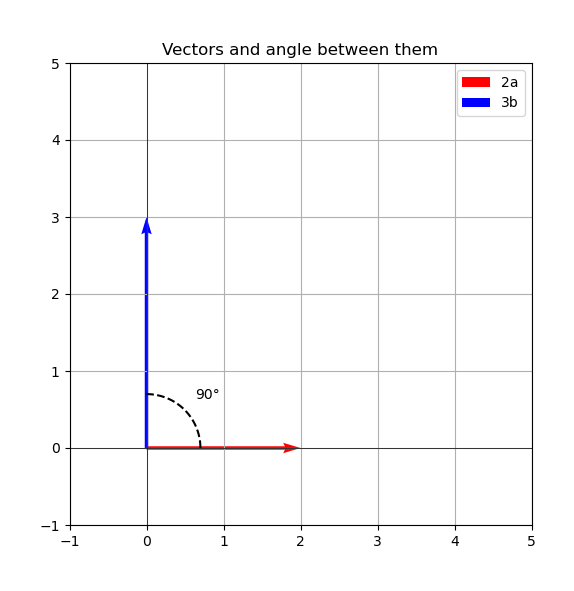
\includegraphics[width=0.6\columnwidth]{figs/fig.png}
\end{center}
\caption{}
\label{fig:Fig1}
\end{figure}
\end{document}